% ---------------------------------------------------------------------
% ---------------------------------------------------------------------
% ---------------------------------------------------------------------

\chapter[Introduction]{Introduction}
\label{chap:intro}

Networks are fundamental in science because they provide a way to model complex systems and relationships between entities. By representing entities as nodes and connections between them as edges, networks can help researchers understand how information, energy, materials, and other resources flow through a system, identify patterns and structures within the data, and make predictions about system behavior. Many real life problems can be modeled as networks or graphs and that is why they are used in many fields, including biology, physics, sociology, and computer science, and have led to significant advances in our understanding of the world around us.

\section{Mathematical notation}
\label{sec:graph}
A network or graph in mathematical literature is, in its simplest form, a collection of interconnected nodes or vertices that represent entities, and the connections or edges between these nodes that represent relationships or interactions between the entities. Graphs are usually described using a combination of mathematical notation and visual diagrams to provide a complete representation of the network structure and properties. The \emph{adjacency matrix} of a network with $N$ nodes is defined as $\mathbf{A}\in\mathbb{R}^{N\times N}$ with elements such as:

\begin{equation}
  A_{ij} =
    \begin{cases}
      1 & \text{if there is an edge between nodes $i$ and $j$}\\
      0 & \text{otherwise}
    \end{cases}       
\end{equation}

Additionally, graphs can be represented visually using a diagram, where nodes are represented as points and edges are represented as lines connecting the points. The direction of the edges (\textit{directed} or \textit{undirected}) and the presence of loops (edges connecting a node to itself) can also be indicated in the visual representation.

It is also worth mentioning other relevant network properties of graph theory as:

\begin{itemize}
  \item \textit{Weighted networks}: A weighted network is a graph in which each edge has a weight or strength assigned to it. These weights represent the strength or importance of the connections between nodes. \textit{Unweighted networks} are those when no weight is assigned.
  \item \textit{Static networks}: A static network is a network that does not change over time. The relationships and connections between nodes are fixed and remain constant. 
  \item \textit{Dynamic networks}: A dynamic network is a network that changes over time. The relationships and connections between nodes can evolve and alter, resulting in a continually changing network structure.
\end{itemize}

Linear algebra will also play a significant role in network analysis as graphs can be represented as matrices. The analysis of networks often involves solving linear systems, determining eigenvalues and eigenvectors, and evaluating matrix functions. Additionally, the examination of dynamic processes on graphs will create systems of differential equations based on their structure. The behavior of the solution over time is highly impacted by that graph's structure (topology), which is reflected in the spectral properties of the matrices related to the graph. That is why one of the most basic questions about network structure is the identification of the relevant nodes in a network which leads us to the concept of centrality.

\section{Centrality measures}
\label{sec:centra}
 Centrality measures are metrics that are used to quantify the relative importance or influence of a node in a network. Indicators of centrality assign numbers or rankings, the higher the more important, to nodes within a graph corresponding to their network position based on different criteria giving rise to several types of centrality measures:

\subsection*{Degree Centrality} Measures the number of connections a node $i$ has to other nodes in the network or what is called degree of a vertex in a graph ($k$), if we define $\mathbf{x}=(x_1,x_2,\dots,x_N)$ as the centrality vector of the graph then: 

\begin{equation}
    x_i^{(deg)}=k_i=\sum_{j=1}^{N}A_{ij}
\end{equation}
This measure is usually normalized by the maximal possible degree, $N − 1$, to obtain a number between 0 and 1. For certain networks, Degree Centrality can be very illuminating as it provides a straightforward and simple indication of a node's connectedness or level of popularity, but fails to consider other crucial elements of the network's structure as node's place within it or its importance.

\subsection*{Closeness Centrality} In order to extend the basic measure of degree and take into account the position of the nodes in the network, closeness and betweeness measures are defined. For its part, Closeness Centrality measures the average distance ($\sum_{j}^{}d(i,j)$) between a node and all other nodes in the network, in the normalized version it can be expressed as:

\begin{equation}
    x_i^{(clos)}= \frac{N-1}{\sum_{j\ne i}^{}d(i,j)}
\end{equation}
An alternative measure of Closeness Centrality is the \textit{Harmonic Centrality} which aggregates distances differently as the sum of all inverses
of distances, ($\sum_{j}^{}1/d(i,j)$). This avoids having a few nodes for which there is a large or infinite distance drive the measurement:

\begin{equation}
    x_i^{(har)}= \frac{1}{N-1}\sum_{j\ne i}^{}\frac{1}{d(i,j)}
\end{equation}

\subsection*{Betweenness Centrality} Measures the number of times a node acts as a bridge along the shortest path between two other nodes in the network. Formally, if we redefine $g_{jk}^i$ to be the number of shortest paths from $j$ to $k$ that pass through $i$ and we define $g_{jk}$ to be the total number of shortest paths from $j$ to $k$, then the Betweenness Centrality of node $i$ on a general network is:

\begin{equation}
    x_i^{(bet)}= \sum_{j<k}^{}\frac{g_{jk}^i}{g_{jk}}
\end{equation}

\subsection*{Eigenvector Centrality} Measures the influence of a node based on the influence of its neighbors. Unlike Degree Centrality which assigns one point for each network connection, Eigenvector Centrality assigns points based on the centrality scores of a node's neighbors, resulting in a more nuanced understanding of a node's centrality. If we denote the centrality of vertex $i$ by $x_i$ where $x$ is the centrality vector, then making use of the adjacency matrix and making $x_i$ proportional to the average of the centralities of $i$’s network neighbours we have for undirected networks:

\begin{equation}
    x_i= \kappa\sum_{j=1}^{N}A_{ij}x_j
\end{equation}
where $\kappa$ is a constant. We can rewrite this equation in matrix form considering $\kappa=1/\lambda$ as

\begin{equation}
    \lambda \mathbf{x} = \mathbf{A}\mathbf{x}
\end{equation}
Hence, $\mathbf{x}$ is an eigenvector of the adjacency matrix for the eigenvalue $\lambda$. Assuming that we wish the centralities to be non-negative, it is shown by the Perron–Frobenius theorem [ref], which states that for a matrix with all elements non-negative, like the adjacency matrix, there is only one eigenvector that also has all elements non-negative, and that is the leading eigenvector. Thus, $\lambda$ must be the largest eigenvalue of the adjacency matrix and $\mathbf{x}$ the corresponding eigenvector. 

Drawbacks of this type of measure, among others, are that it does not scale well for directed networks without certain modifications or even worse it is not applicable in acyclic networks, i.e., directed graphs with no loops. There are a number of variants of Eigenvector Centrality that address these
problems like Katz centrality and PageRank.

\subsection*{Katz Centrality}
Katz Centrality will be covered to a greater extent in section~\ref{sec:back} as it is central topic of this thesis but only mentioning that it is a centrality measure that is based on the idea that a node's importance depends on both its direct connections and the connections of its neighbors. The computation of this centrality score will lead to the resolvent matrix of $\mathbf{A}$, the adjacency matrix, which can be interpreted as an infinite weighted sum of the number of paths of all lengths from the node to all other nodes in the network. The weights in this sum decrease exponentially with the length of the path, so that longer paths are given less importance which reflects the idea that a node's influence decreases as the distance from it increases. 


\subsection*{Page Rank}

The Katz centrality measure discussed earlier has a potential flaw. If a node with a high Katz score has links to many other nodes, then all of those linked nodes will also receive a high centrality score. PageRank, instead, is a variant in which the centrality derived from network neighbors is proportional to their centrality divided by their out-degree. Therefore, nodes that point to many others pass only a small amount of centrality on to each of those others, even if their own centrality is high.

In mathematical terms, this centrality is defined by:

\begin{equation}
\label{eqn:pr1}
    x_i= \alpha\sum_{j=1}^{N}A_{ij}\frac{x_j}{k_j^{\text{out}}} + \beta
\end{equation}
where $\mathbf{A}$ is the adjacency matrix and $\alpha$, $\beta$ are positive free parameters as in Katz Centrality --ref--.

Setting $k_j^{\text{out}}=1$ to avoid zero-division for nodes with no outgoing edges we can express eq. (\ref{eqn:pr1}) in matrix form:

\begin{equation}
\label{eqn:pr2}
    \mathbf{x} = \alpha\mathbf{AD^{-1}x} + \beta \mathbf{1}
\end{equation}
with $\mathbf{1}$ being the vector of ones $(1,\dots,1)$ and $\mathbf{D}$ being the diagonal matrix with elements $D_{ii} = max(k_i^{\text{out}},1)$. Rearranging for $\mathbf{x}$ and setting the conventional value of $\beta=1$, the PageRank centrality yields:
\begin{equation}
\label{eqn:pr3}
    \mathbf{x} = (\mathbf{I} - \alpha\mathbf{AD^{-1}})^{-1} \mathbf{1}
\end{equation}
with $0<\alpha<1$, it should be less than the inverse of the largest eigenvalue of $\mathbf{AD}^{-1}$ (Google uses $\alpha = 0.85$).


PageRank was developed by Google co-founders Larry Page and Sergey Brin as a way to rank websites in their search engine results. The basic idea behind PageRank is that a node is considered important if it is linked to by many other important nodes. The PageRank score of a node is determined by the sum of the PageRank scores of the nodes that link to it, with a damping factor applied to reduce the influence of nodes with many outbound links. PageRank centrality is widely used in the field of network analysis and has been applied to a wide range of networks, including the World Wide Web, social networks, and biological networks.


Each centrality measure provides a different perspective on the importance of a node in a network and can be useful in various applications, such as network analysis, recommendation systems, or identifying key players in complex systems. The most appropriate centrality measure will require the analysis of the specific characteristics of our network.

\begin{figure}[htbp]\centering
	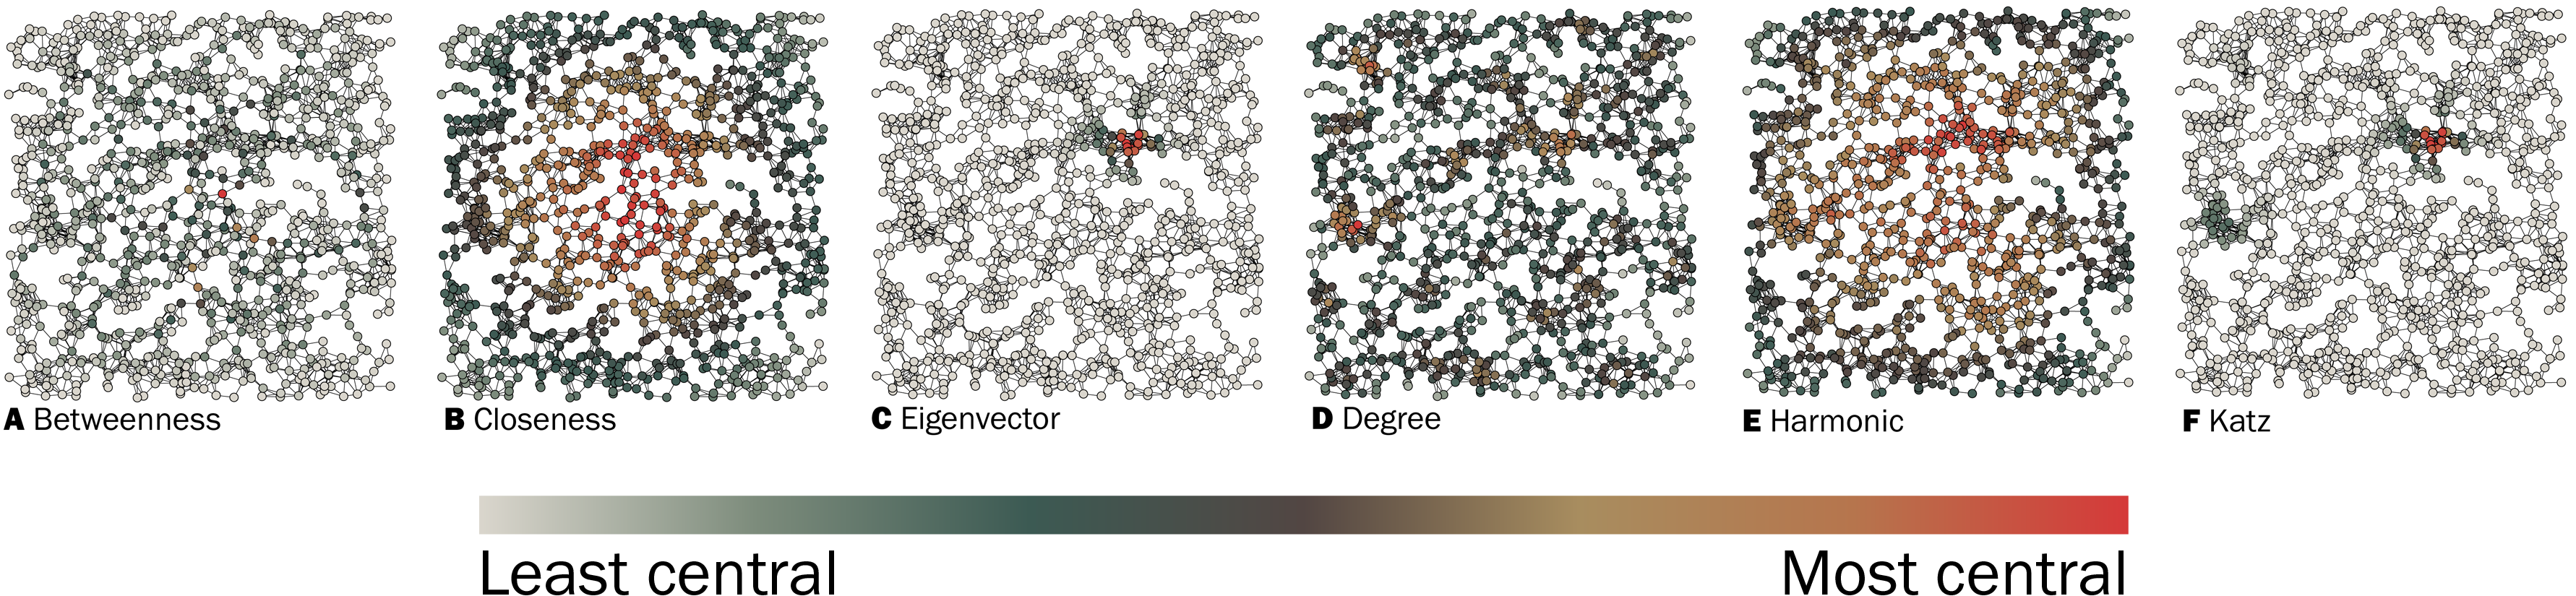
\includegraphics[width=.93\textwidth]{centrality}
	\caption{Examples of A) Betweenness centrality, B) Closeness centrality, C) Eigenvector centrality, D) Degree centrality, E) Harmonic centrality and F) Katz centrality of the same random geometric graph.}
	\label{centrality}
	\bigskip
\end{figure}

\section{Background on Katz centrality in static networks}
\label{sec:back}
Text.

\section{Motivation of the study}
\label{sec:motiv}
Text.


Lacus viverra vitae congue eu consequat ac felis donec. Ultrices dui sapien eget mi proin sed libero enim. Id consectetur purus ut faucibus pulvinar elementum integer\index{Integer}. In massa tempor nec feugiat \textsl{Newman} \cite{newman2018networks}.
% ---------------------------------------------------------------------
% ---------------------------------------------------------------------
